%**********************************************************
\subsection{Task Overview}
One can define and describe briefly how the gateway is implemented, making use of threads and processes.

\begin{itemize}
	\item \textbf{tLoraRecv: } receives all messages from local systems, using LoRa communication;
	\item \textbf{tTCPRecv: } receives all messages from the remote server, using TCP-IP communication;	
	\item \textbf{tLoraSend: } sends all received messages from the remote server, in textit{tTCPRecv}, to the local systems, using LoRa communication;
	\item \textbf{tTCPSend: } sends all received messages from local systems, in \textit{tLoraRecv}, to the remote server, using TCP-IP communication;
\end{itemize}

One can define the relationship between the tasks as follows, in figure \ref{fig:gwOverview}. To communicate the local system received messages and the remote server sender service its used a vector of messages, named \textit{msgs\_to\_rs}. In the communication between the remote server received messages and the local system sender service its also used a vector of messages, named \textit{msgs\_to\_ls}.

\begin{figure}[H]
	\centering
	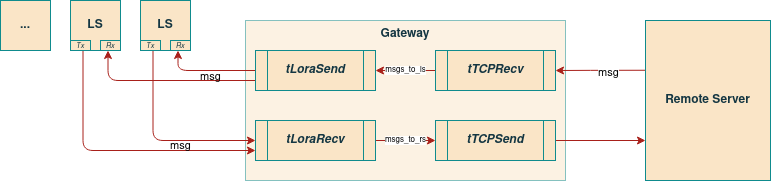
\includegraphics[width=1\textwidth]{09sw_specification/gwOverview}
	\caption{Gateway Overview.}
	\label{fig:gwOverview}
\end{figure}

%**********************************************************
\clearpage
\subsection{Task Priority}
The priority assignment diagram for the gateway is represented in figure \ref{fig:gwt_priority}.

\begin{figure}[H]
	\centering
	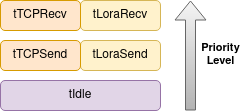
\includegraphics[width=0.5\textwidth]{09sw_specification/gwt_priority}
	\caption{Gateway Priority Assignment Schematic.}
	\label{fig:gwt_priority}
\end{figure}

%**********************************************************
\subsection{Task Synchronization}

\myparagraph{Condition Variables}
The condition variables used in this system are listed below.

\begin{itemize}
	\item \textbf{condLoraSend:} used to notify \textit{tLoraSend} that a new message is ready to be sent;
	\item \textbf{condTCPSend:} used to notify \textit{tTCPSend} that a new message is ready to be sent;
\end{itemize}

\myparagraph{Mutexes}
The mutexes used in this system are listed bellow.

\begin{itemize}
	\item \textbf{mutLoraComm:} used to protect the LoRa communications (send and receive);
	\item \textbf{mutLoraSend:}	used to protect the handling of the vector \textit{msgs\_to\_ls};
	
	\item \textbf{mutTCPComm:} used to protect the TCP/IP communications (send and receive);
	\item \textbf{mutTCPSend:} used to protect the handling of the vector \textit{msgs\_to\_rs}.
\end{itemize}

\subsection{Task Communication}
In order to communicate all messages between the LoRa related tasks and the TCP related tasks are used two vectors of strings, \textit{msgs\_to\_rs} and \textit{msgs\_to\_ls}. This belongs to the container library \textit{std::vector} from C++ libraries, which implements a dynamic contiguous array. The storage of the vector is handled automatically being expanded and contracted as needed. This provides functions like \textit{push\_back()}, \textit{insert()} or \textit{pop\_back()} which allows to insert or remove new elements as needed.

%**********************************************************
\subsection{Flowcharts}
Each local system has a predefined ID, which may be presented in a physical label for an operator to use this information. When a local system is being installed, it will use it's predefined ID in all communications with the remote server until the operator registers the local system that's being installed, in the remote server. By doing this, the remote server assigns a new ID to the local system, which is then sent to the local system, for this to be used in further communications.

\myparagraph{tLoraRecv}
This task, presented in figure \ref{fig:gwtLoraRecv}, is responsible for receiving all the packets sent by the local systems, through LoRa communication. This task makes use of a mutex \textit{mutLoraComm}, to protect LoRa send and receive functions, which must not occur at the same time. Besides that, it uses a mutex \textit{mutTCPSend} to protect the vector of messages \textit{msgs\_to\_rs} which can be changed in \textit{tTCPRecv}.

When a message is received it is pushed into the vector of messages \textit{msgs\_to\_rs}, to be sent to the remote system. This way, we can receive continually messages from local systems, while there is another task sending this messages. This operation is protected by \textit{mutTCPSend}. After the message is added to the vector of messages, this task signals the task \textit{tTPCSend} through the condition variable \textit{condTCPSend}, in order for this to send the newly added message to the remote system.

\begin{figure}[H]
	\centering
	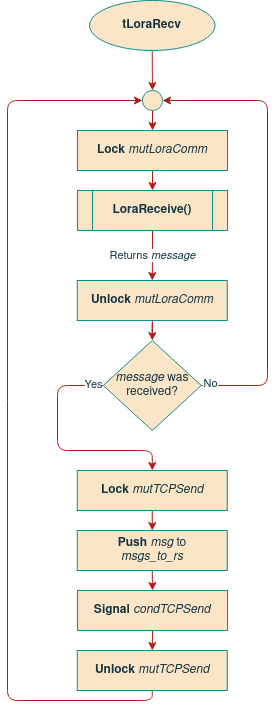
\includegraphics[width=.5\textwidth]{09sw_specification/gwtLoraRecv}
	\caption{Flowchart: Gateway tLoraRecv.}
	\label{fig:gwtLoraRecv}
\end{figure}

\myparagraph{tLoraSend}
This task, presented in figure \ref{fig:gwtLoraSend}, is responsible for sending all the packets sent by the remote system to the local systems. In addiction to the mutex \textit{mutLoraComm}, this task makes use of another mutex \textit{mutLoraSend}, which comes along with the condition variable \textit{condLoraSend}, in order to protect the insertion and removal of messages from the vector \textit{msgs\_to\_ls}.

When there are no messages to send to the local systems, i.e, the messages vector \textit{msgs\_to\_ls} is empty, then the task enters a sleep state, waiting for \textit{condLoraSend} to be notified. When this happens, the mutex that protects LoRa communication is locked and a message is popped from the queue of messages to being sent to the local systems. If the vector \textit{msgs\_to\_ls} is not empty after sending a message, this task continues to do so until there are no more to send, before entering into sleep state again.

\begin{figure}[H]
	\centering
		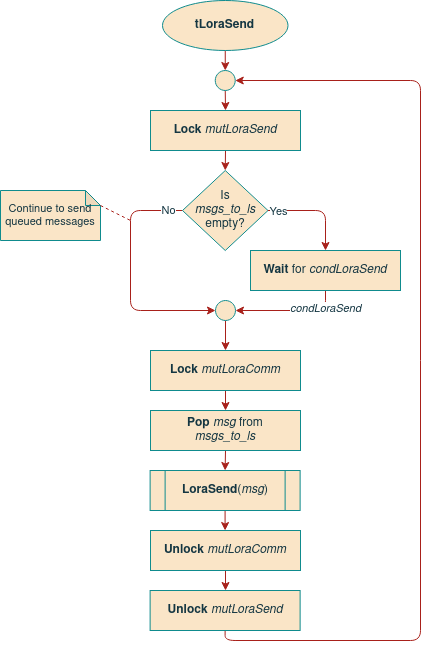
\includegraphics[width=.8\textwidth]{09sw_specification/gwtLoraSend}
	\caption{Flowchart: Gateway tLoraSend.}
	\label{fig:gwtLoraSend}
\end{figure}

\myparagraph{tTCPSend}
This task, presented in figure \ref{fig:gwtTCPSend}, is responsible for sending all the messages sent by the local systems to the remote system, being received by in the task \textit{tLoraRecv}. It uses two mutexes: \textit{mutTCPSend} associated with the condition variable \textit{condTCPSend}, that synchronizes the insertion and removal of the messages from the vector \textit{msgs\_to\_rs}; and \textit{mutTCPComm}, to protect the communications send and receive.

When there are no messages to send to the remote system, i.e, the messages vector \textit{msgs\_to\_rs} is empty, the task enters a sleep state, waiting for \textit{condTCPSend} to be notified by the task receiving messages from the local systems. When messages are received, the vector \textit{msgs\_to\_rs} is not empty, and one can lock the mutex \textit{mutTCPSend} in order to pop a message from the vector. After that, one can send the message via TCP/IP communication protocol, protecting the communication with the mutex \textit{mutTCPComm}.

\begin{figure}[H]
	\centering
	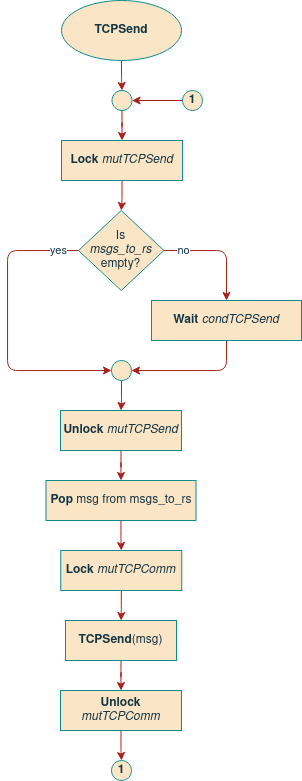
\includegraphics[width=.4\textwidth]{09sw_specification/gwtTCPSend}
	\caption{Flowchart: Gateway tTCPSend.}
	\label{fig:gwtTCPSend}
\end{figure}

\myparagraph{tTCPRecv}
This task, presented in figure \ref{fig:gwtTCPRecv}, is responsible for receiving the messages sent by the remote system to the local systems. Unlike the send tasks, this thread never enters the sleep state because we can receive a message at any moment, so first, one have to lock the mutex \textit{mutTCPComm} and try to receive a message. If it was received a message, i.e, the \textit{msg} variable is not empty, then one can push the message to the messages vector \textit{msgs\_to\_ls} and notify the condition variable \textit{condLoraSend}, after locking its mutex \textit{mutLoraSend}, to inform that a new message has been received.

\begin{figure}[H]
	\centering
	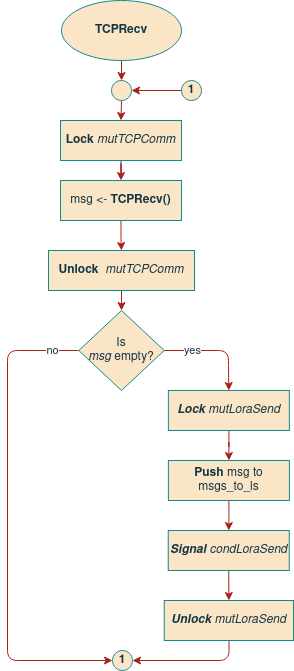
\includegraphics[width=.4\textwidth]{09sw_specification/gwtTCPRecv}
	\caption{Flowchart: Gateway tTCPRecv.}
	\label{fig:gwtTCPRecv}
\end{figure}

%%**********************************************************
\subsection{Start-up Process}
% create TCP IP and LORA
%%**********************************************************
%\subsection{Shutdown Process}
